\documentclass[10pt,oneside]{article}
\usepackage{graphicx}
\usepackage{url}
\usepackage{hyperref}
\usepackage{multirow}
\usepackage{algorithm}
\usepackage{algorithmic}
\usepackage{caption}
\usepackage{comment}
\hypersetup{
	colorlinks=true,
	citecolor=blue,%
    filecolor=blue,%
    linkcolor=blue,%
    urlcolor=blue
}


\DeclareCaptionFormat{myformat}{#3}
\captionsetup[algorithm]{format=myformat}

\newcommand{\doctitle}{%
Graph Coloring}
\newcommand{\cmnt}[1]{}

\pagestyle{myheadings}
\markright{\doctitle\hfill}
%\markboth{\hfill\doctitle}{\doctitle\hfill}

\bibliographystyle{siam}

\addtolength{\textwidth}{1.00in}
\addtolength{\textheight}{1.00in}
\addtolength{\evensidemargin}{-1.00in}
\addtolength{\oddsidemargin}{-0.00in}
\addtolength{\topmargin}{-.50in}

\hyphenation{in-de-pen-dent}
\date{University of Illinois, Urbana-Champaign} %hack.

%\title{\textbf{\doctitle}\\
\title{\textbf{Graph Coloring Using State Space Search}}

\begin{comment}
\author{Sandeep Dasgupta\thanks{Electronic address: \texttt{sdasgup3@illinois.edu}}
\qquad Tanmay Gangwani\thanks{Electronic address: \texttt{gangwan2@illinois.edu}}
\qquad Mengjia Yan\thanks{Electronic address: \texttt{mengjia@illinois.edu}}
\qquad  Novi Singh \thanks{Electronic address: \texttt{novi.singh94@gmail.com}}} 
\end{comment}

\author{Sandeep Dasgupta 
\qquad Tanmay Gangwani
\qquad Mengjia Yan
\qquad  Novi Singh}

\begin{document}

\thispagestyle{empty}

\maketitle
\section{Introduction}
As a subject with many applications, graph coloring is one of the most studied
  NP-hard problems. Due to its time complexity, graph coloring is an excellent
  candidate for implementation with a parallelized architecture, and as such
  has become our choice for our project. Of the many ways that graph coloring
  can be adapted for parallel programming there are two main approaches in
  literature: the iterative and state-space search methods.  The iterative
  approach begins by dividing the vertices of the graph to be colored into
  different groups, each of which is assigned to a node in the cluster. 
  In the context of Charm++, this would be akin to dividing the vertices
  among a set of chares. At this point each chare would independently color its
  assigned vertices, and once all vertices had been colored the chares would
  communicate with each other to see if each of their respective vertices had
  any neighbors on other chares that violate the constraints of the coloring
  problem. Once color conflicts have been assessed, the chares would seek to
  mediate these problems through another round of independent coloring among
  the chares, a process that would be repeated until the graph has been
  successfully colored or shown to be uncolorable with the given number of colors. 
  An example implementation is present by Boman et al.~\cite{EuroPar2005}.

  In contrast, the state-space search method seeks to start with the initial
  graph and color it by creating child chares for each possible color
  assignment among the vertices. This process of coloration and child creation
  is repeated until a solution to the coloring problem is found or an
  exhaustive search has yielded no solution. By doing so, the program explores
  all different possible colorations of the graph for a given number of colors. 
  A state-space search exploration could find only the first valid solution and terminate; 
  find all possible solutions; or find the most \emph{optimal} solution among all possibilities.
  Sun et al.~\cite{ParSSSEPPL} have developed a general framework for solving state-space search problems
  like graph coloring and N-Queens.
  
  State-space search has an advantage over the iterative approach in that it
  does not require the large number of message exchanges between chares to
  mediate coloring conflicts. However, the state-space search does require the 
  use of many more chares than the iterative approach and could incur 
  higher memory overhead. Given the Charm runtime features likes load balancing, 
  prioritized message execution and the general emphasis on over-decomposition, 
  we implement the state-space approach for finding the \textbf{first} valid coloring 
  of an input graph, with a given number of colors. 
 
\section{Program Structure}

\begin{algorithm}[h]
\caption{.ci file structure} \label{algo:ci}
\begin{algorithmic}[1]
\STATE \textbf{Main Chare} \\
\qquad Spawn root-node of state space search 

\STATE \textbf{Root-node Chare} \\
\qquad Graph-preprocessing algorithms (precoloring, vertex removal, subgraph detection) \\
\qquad Spawn (child) node chares with value-ordering \\ 
\qquad Wait for response from children \\

\STATE \textbf{Node Chare} \\
\qquad Graph-preprocessing algorithms (vertex removal, subgraph detection) \\
\qquad Depending on grain-size \\
\qquad \qquad Spawn (child) node chares with value-ordering, \emph{or} \\
\qquad \qquad Call sequential coloring algorithm \\
\qquad Wait for response from children (if any) \\ 
\qquad Merge children’s status, propagate response to parent \\

\STATE \textbf{Group Chares} \\
\qquad Collect statistics, terminate search of subtrees or whole process \\

\STATE \textbf{Message Categories} \\
\qquad Bitvector prioritization for node chare seeds \\
\qquad Expedited privilege for result signals \\
\end{algorithmic}
\end{algorithm}

Our implementation of state-space search is outlined in the structure of our
  .ci file. At the start of the program a root node chare is created by the main
  chare. This chare is responsible for preconditioning the input graph for the state-space 
  exploration and is also the chare where the final result is accumulated. Next, the root-node 
  chare selects a graph vertex to color based on heuristics, and spawns further chares which
  form the nodes of the state-space tree. In effect, each chare receives a partially colored graph
  as input and is responsible for finding a valid coloring (if one exists) for the entire graph starting 
  from \emph{that} initial state. It does so by pruning the graph using vertex removal and subgraph 
  detection, and then spawning child chares to further distribute the search. In certain cases 
  (section~\ref{sec:grainsize}), the chare calls a sequential coloring algorithm instead of creating child 
  chares.
  
  We use the Charm++ \emph{group} feature for bookkeeping purposes and for 
  kill-chasing (section~\ref{sec:killchasing}). The spawning of new node chares is loosely ordered 
  using bit-vector prioritization (section~\ref{sec:bitvector}). We used expedited message privileges for
  result messages that flow from leaf nodes of the state-space all the way up to the root node. This prevents
  delays in the termination of the program after a valid first solution has been found to the graph coloring
  problem.
  
\section{Heuristics for State-Space Search}
Due to the NP-hard nature of the problem, the number of all possible states in
  the state-space search is exponential in size, and as such heuristics to
  reduce the number of states that are searched are necessary for any tractable
  computation to be possible. This section outlines the details. The ideas are borrowed 
  from the work of Kale et al.~\cite{Kale1995}.

\subsection{Pre-Coloring}
  The first of these heuristics is a preprocessing technique, namely the
  pre-coloring of the graph. We find the 3-vertex cliques in the graph, and assign
  them the lowest available color ensuring that a vertex does not get any of the colors 
  assigned to its neighbors. However, we found that this technique is best applied to 
  sparse graphs only. As dense graphs tend to have many, many 3-vertex cliques, this preprocessing
  technique often results in an unoptimized sequential coloring of a large part of the input graph.
  This may result in un-colorability of the graph even though it may be colorable with the given number
  of colors by using an optimized approach. 

 \subsection{Vertex Removal}         
            By noting that a vertex with degree less than the number of available colors must
            always have a valid possible coloring, we can remove such a vertex
            from the graph (pushing it onto a local stack), color the rest of the graph, 
            and re-include the removed vertex, assigning it the lowest available color.
            It is important to note that this removal can be performed
            recursively. That is, the removal of a vertex from the graph may
            lower the degree of its neighboring vertices to the point that this
            heuristic could then be applied to them. 
            
\subsection{Next Vertex Selection}
            An intuitive and simple heuristic guides our process for selecting
            the next vertex to be colored. By picking the vertex with the least
            available number of potential colors, we can move more efficiently through the 
            state-space. Two related optimizations include \textbf{impossibility-testing} 
            and \textbf{forced-move}. In the former, if
            after a vertex is colored, one of its neighbors has no available
            colors left, then the state for that coloring is not generated since it can never lead to a valid 
            coloring of the entire graph. The
            latter dictates that after a vertex is colored, if the number of possible
            colors at any neighbor is reduced to 1, then the neighbor is colored in the 
            same step. This process is repeated recursively since the coloring of a
            neighbor might lead to forced-move for the neighbor of the neighbor.

  
\subsection{ValueOrdering \& Bit-vector Prioritization}   
\label{sec:bitvector}
            Value ordering provides a lexicographical ordering of state-space search nodes to
            prioritize some nodes over others. This prioritization is based
            on the fact that the set of configurations resulting from the possible coloring of a 
            graph vertex should be explored in the order of decreasing likelihood of getting a valid coloring for
            the entire graph. The color that needs to be explored first must be the one that affects the neighbors the least.
            To calculate this ordering, we find for each coloring of the vertex, the sum of the number of remaining possible 		   colors for all its neighbors. \emph{Ranks} are assigned to the colors based on the calculated sum - highest rank 		   assigned to the color which results in the maximum sum. Based on this ranking, bit-vector priorities are assigned
            to the newly spawned child chares.
           
            With respect to the state-space tree, this results in the left sibling of a node chare having a higher
            priority than the right sibling, leading to a \emph{broom-stick sweep}. Chare seeds are picked up 
            by the Charm scheduler based on their priority. This adds some notion of determinism 
            in the otherwise non-deterministic exploration. It also provides relatively consistent (monotonic) 
            speedups as the number of available PEs is increased. This idea has been presented by Saletore et al.~\cite{SearchAAAI90}.
          
\subsection{Grain-size Control}   
\label{sec:grainsize}
  In Charm terminology, grain-size is the amount of work done by each chare. For the graph 
  coloring problem, this corresponds to the number of vertices colored by each chare. Non-leaf chares 
  in the state-space subtree perform minimal amount of work by coloring a single vertex only, and spawning 
  more chares to work on its behalf. For our experiments, we define grain-size as a threshold $G$. If 
  the number of uncolored vertices at a chare falls below $G$, then instead of creating new chares, the 
  chare become a leaf node and colors the remaining subtree locally.
  
  We use grain-size as a parameter to determine the number of chares created in the system.
  Picking close to optimal grain-size is of paramount importance; too
  low and a huge number of chares are generated, incurring parallelization
  overhead, and a threshold that is too high results in very few chares and an
  under-utilization of processing power. 
  
  The sequential algorithm run at each leaf chare is a stack based, worklist
  approach that employs vertex removal and value ordering. In some cases, the 
  sequential algorithm could take an excessive amount of time to explore the entire subtree of nodes.
  The large entry method could hog the PE leading to undesirable effects. To mitigate this, the
  sequential coloring is made \textbf{pre-emptable}, which is to say that the coloring method
  returns after a set timeout value. A new call to the sequential coloring method is 
  inserted in the scheduler queue at the same PE. On invocation, the method picks 
  off from where it left at the time of preemption. By doing this, we prevent the 
  blocking of expedited messages, such as
  success or failure messages, and don't unnecessarily delay the termination of
  the program. 
  
  An important note to the selection of grain size is that it had
  to be manually fine-tuned to find a good value as variations in graph
  structure and edge density would result in vastly different grain size
  optimums.

\subsection{Detection of Independent Subgraphs}   
This heuristic is to detect independent subgraphs, an , $\mathcal{O}(V+E)$
operation, in the input graph and then to run the coloring algorithm on each
subgraph separately.  By splitting the graph into two or more disconnected pieces,
we often obtain large speedups as the problem is exponential in nature and
evaluating multiple smaller subgraphs results in extremely fewer possible states
as compared to evaluating a single, larger graph. 

This heuristic also leads to a changing of the structure of the state-space tree 
in that it transforms it into an AND-OR tree. In the single graph approach, 
either the left OR right subtree (or at least one of many) has to find a solution 
to the coloring problem for an overall solution to be found, and failure in one subtree
does not necessitate the failure of the entire search. However, in the case of an AND-OR tree, when
splitting the problem into multiple, independent subgraphs it becomes necessary
for a solution to exist for all of the subgraphs (the left AND right subtrees
    have to yield solutions), and failure for any one subgraph implies failure for
  the entire search. Additionally, higher priority is given to that subtree of an
    AND node which has less uncolored vertices, with the hope that it would finish faster. 

  \section{Kill Chasing}
   \label{sec:killchasing}  
    There are conditions under which a node chare should be prohibited from spawning new chares. The issue of
    delivering the prohibition signal before the actual spawning is referred to as kill-chasing.
    We employ group chares to prevent the spawning of new chares
    if a solution to the graph coloring problem has been determined in some part of the state-space search tree. 
    Before creating any children, a chare must obtain \emph{permission} from the group chare on its PE. 
    When a solution is found in the system, all the group chares are notified immediately with expedited messages, 
    and prevent any node chares from further creating progenies. Similarly, in the case of an AND node, if one of the
    subtree reports a failed coloring, the information is broad-casted to the group chares, and node chares in the sibling 
    subtrees are prevented from creating further chares.

\section{Setup}

  Table~\ref{tb:1} shows the graphs along with their features which
  we used for our experimentations. 
  Each of the graphs, G1-G6, were randomly generated by a python script. We
  varied the number of vertices, average edge density, and maximum number of
  allowed colors, and additionally generated both truly random graphs and graph
  that were composed of two or more independent subgraphs. All of the graphs in
  the table were colorable save for two. Graphs G5 and G6 have subgraph partitions.

  All runs were done using 12 PEs on the Taub campus cluster. For each configuration,
  we report the average of 3 runs.

\begin{table}[h]
\centering
\begin{tabular}{|l|l|l|l|l|}
\hline
   & Vertices & Edge Density & \#Colors &  Colorable   \\ \hline
G1 & 300      & 12           & 9        & Yes \\ \hline
G2 & 300      & 8            & 4        & No  \\ \hline
G3 & 1000     & 5            & 5        & Yes \\ \hline
G4 & 500      & 7            & 6        & Yes \\ \hline
G5 & 1000     & 6            & 6        & Yes \\ \hline
G6 & 450      & 6            & 5        & No \\ \hline
\end{tabular}
\caption{Summary Of Graphs}
\label{tb:1}
\end{table}

\section{Results}

\begin{table}[h]
  \scalebox{0.8} {
    \begin{tabular}{|c|c|c|c|c|c|c|c|c|}
    \hline
                        & Vertices              & Grain Size           & Timeout             & Priority Bits           & Value Ordering          & Sub-graph Detection     & Execution Time (s) & \#Chares \\ \hline
    \multirow{2}{*}{G1} & \multirow{2}{*}{300}  & \multirow{2}{*}{290} & \multirow{2}{*}{10} & Enable                  & \multirow{2}{*}{Enable} & \multirow{2}{*}{Enable} & 18                 & 1220     \\ \cline{5-5} \cline{8-9} 
                        &                       &                      &                     & Disable                 &                         &                         & 31                 & 189105   \\ \hline
    \multirow{4}{*}{G2} & \multirow{4}{*}{300}  & 260                  & \multirow{4}{*}{10} & \multirow{4}{*}{Enable} & \multirow{4}{*}{}       & \multirow{4}{*}{}       & 27                 & 186329   \\ \cline{3-3} \cline{8-9} 
                        &                       & 280                  &                     &                         &                         &                         & 16                 & 124601   \\ \cline{3-3} \cline{8-9} 
                        &                       & 290                  &                     &                         &                         &                         & 7                  & 2681     \\ \cline{3-3} \cline{8-9} 
                        &                       & 300                  &                     &                         &                         &                         & 82                 & 1        \\ \hline
    \multirow{2}{*}{G3} & \multirow{2}{*}{1000} & \multirow{2}{*}{960} & 10                  & \multirow{2}{*}{Enable} & \multirow{2}{*}{Enable} & \multirow{2}{*}{Enable} & 41                 & 235      \\ \cline{4-4} \cline{8-9} 
                        &                       &                      & 30                  &                         &                         &                         & 214                & 585      \\ \hline
    \multirow{2}{*}{G4} & \multirow{2}{*}{500}  & \multirow{2}{*}{480} & \multirow{2}{*}{10} & \multirow{2}{*}{Enable} & Enable                  & \multirow{2}{*}{Enable} & 102                & 642      \\ \cline{6-6} \cline{8-9} 
                        &                       &                      &                     &                         & Disable                 &                         & 133                & 669      \\ \hline
    \multirow{2}{*}{G5} & \multirow{2}{*}{1000} & \multirow{2}{*}{960} & \multirow{2}{*}{5}  & \multirow{2}{*}{Enable} & \multirow{2}{*}{Enable} & Enable                  & 0.01               & 4        \\ \cline{7-9} 
                        &                       &                      &                     &                         &                         & Disable                 & 35                 & 2610     \\ \hline
    \multirow{2}{*}{G6} & \multirow{2}{*}{450}  & \multirow{2}{*}{410} & \multirow{2}{*}{5}  & \multirow{2}{*}{Enable} & \multirow{2}{*}{Enable} & Enable                  & 0.02           & 4        \\ \cline{7-9} 
                        &                       &                      &                     &                         &                         & Disable                 & 5.77           & 49646    \\ \hline
    \end{tabular}
  }
\caption{Performance Data}
\label{tb:2}
\end{table}

The performance data is summarized in Table~\ref{tb:2}. The columns in the table refer to the configurable knobs in the program. For each of the graphs, we toggle some feature (heuristic), and measure the impact. We report the 
application running time in seconds, and the number of chares created in the system. Time is measured using \emph{CkTimer} functionality, and the number of chares are calculated using groups.

For G1, enabling bit-vector prioritization improves performance by 1.7x. This is because bit-vector prioritization
directs the state-space exploration to a path with a high likelihood of a solution. In G2, we evaluate the impact of changing the grain size for a graph with 300 vertices. A grain size of 300 is akin to 
sequential coloring, and is completed in 82s. As the grain size is varied from 260 to 290, the performance improves. This is because increasing grain size results in lesser number of chares being created, and hence lesser parallelism overheads. For G3, we varied the time for which the sequential coloring algorithm is allowed to run uninterrupted. We observed that changing the value from 30s to 10s results in a performance improvement of 5.2x. This is because a lower timeout value results in speedy delivery of the success (or failure) messages from the leaf chare to the root chare, resulting in prompt termination of the program. G4 shows the effect of using the value ordering heuristic. Ordering the configurations resulting from the coloring of a particular vertex leads to an improvement of 1.3x. Graphs
G5 and G6 present the huge potential of subgraph detection. G5 and G6 are partitioned graphs. For the scenario with subgraph detection disabled, the application creates many chares which explore the state-space. This incurs some parallelization overhead. With subgraph detection enabled, the partitions (subgraphs) are colored sequentially since the number of uncolored vertices in each partition falls below the grain size. This results in the creation of just 4 chares - one root chare, and one each for the 3 partitions in G5 and G6.  

\section{Seed Balancer}
To further improve the execution time and processor utilization in our program,
  we sought to employ a seed balancer. This balancer divides the creation of
  new chares across processors to even out the distribution of the workload.
  More specifically, we tried ``work stealing'' and ``NeighborLB'' as strategies
  for the seed balancer. In the case of the former, we found little difference in processor
    utilization compared to an execution without a seed balancer, but for the latter we
      were able to note a major difference. In Figure~\ref{fig_sdb}(b), generated
      using Projections, utilization remains higher for a longer period of time
      with NeighborLB enabled as compared to without a seed balancer,
           Figure~\ref{fig_sdb}(a).  Figure~\ref{fig_chare_dist} shows the distribution of the 
           chares across the PEs with and without the seed balancer. Without the seed balancer, 
           all the PEs get roughly the same number of chares. This ultimately leads to lower overall
           processor utilization since some leaf chares take more time to complete than others. A 
           seed balancer can sense such un-evenness and migrate more seeds away from a processor
           where the leaf chares have a longer execution time. This results in some PEs getting more chares
           than others --- PE9 gets more 1000 more chares than PE7 --- but the overall processor utilization is 
           improved, and application time reduced.
        
\begin{figure}[h]
\centering
\begin{tabular}{c c}
  \scalebox{0.3}{
    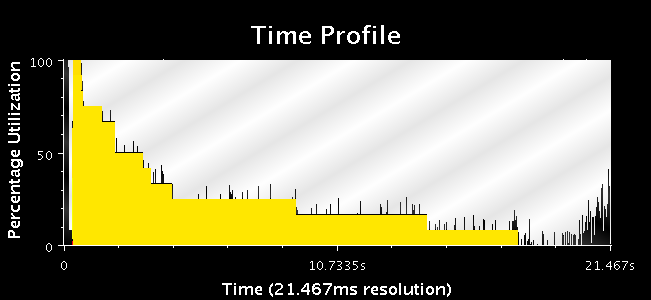
\includegraphics{1.png}
  }
& 
  \scalebox{0.3}{
    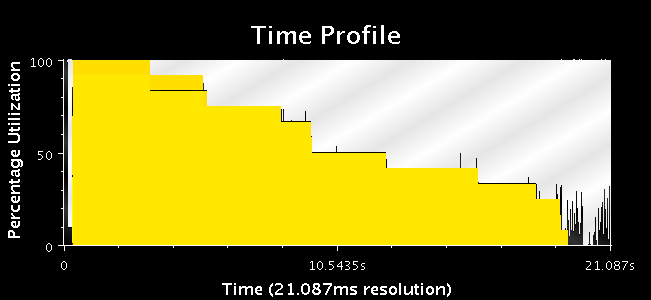
\includegraphics{2.png}
  } \\
\qquad (a) & \quad (b) \\
\end{tabular}
\caption{Percentage Utilization on graph G2 with grainsize 260, timeout = 10s   (a) Without Seed balancer (b) With ``NeighborLB'' Seed Balancer}
\label{fig_sdb}
\end{figure}            

\begin{figure}[h]
\centering
  \scalebox{0.5}{
    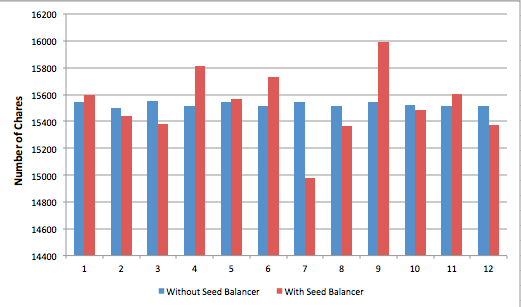
\includegraphics{3.png}
  }
\caption{Distribution of seeds on each of the 12 PEs}
\label{fig_chare_dist}
\end{figure}            


\section{Core Scaling}

\begin{figure}
\centering
  \scalebox{0.8}{
    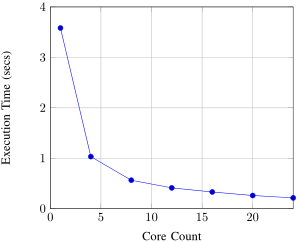
\includegraphics{core_count.png}
  }
\caption{Graph G2, with 4 colors - vertices 300, edge-density 8  }
\label{fig_core_scale}
\end{figure}            

  For an  un-colorable graph with no subgraphs (such as G2), all the states need to be 
  explored before a failure can be reported. Adding cores is useful is such a scenario since
  the state-space exploration work gets distributed. As shown in Figure~\ref{fig_core_scale}, 
  the execution time for G2 reduces with increasing core count. We observe diminishing returns
  after adding a certain number of PEs. This could be attributed to that fact with more PEs, the ancestry
  of a particular node in the state-space subtree could be spread out among different PEs, leading to 
  more network overheads as result signals propagate from children to parent.
  
  For colorable graphs, we could not establish a consistent trend with increasing number of PEs. We observe
  that the entire state-space is not explored for a colorable graph, unlike an un-colorable one. Adding more 
  processors, hence, is not expected to yield the same benefits. Secondly, our heuristics are strong enough to guide 
  the search towards a successful coloring. Since our implementation terminates after the first solution, work done by
  extra processors is not always required. Moreover, the extra processors could add useless work on the path of 
  the processor which ultimately produces the first coloring, and hence may negatively impact the overall application
  execution time. We attribute the observed discrepancies to these effect. Bit-vector prioritization, in theory, helps to 
  obtain monotonic speedups with additional processors. We note, however, that to work perfectly, such a solution 
  would require a system with a \textbf{central} scheduling queue for the chare seeds. 

\section{Conclusion}
Our project sought to employ as many heuristics as possible to mitigate the
  exponential nature of the graph coloring problem, and this desire combined
  with experimentation of other execution parameters has allowed us to create
  an effective program for graph coloring. Many of our difficulties lay in
  fine-tuning our heuristics to work with the large variation in graph
  structure that could occur, as well as working with the non-deterministic
  effects in the exploration of the state-space tree. In the future, this work
  could be expanded upon to more clearly express the impact of each heuristic
  on a graph, and to change the application of certain heuristics (for example, grain-size)
  automatically depending on the characteristics of the graph.

\nocite{*}
\bibliography{CS598_project_proposal}

\end{document}
